\documentclass[border=2pt]{standalone}
\usepackage{tikz}
\usetikzlibrary{positioning, fit, shapes, arrows, calc}

\pgfdeclarelayer{bg}    % declare background layer
\pgfsetlayers{bg,main}  % set the order of the layers (main is the standard layer)

\newcommand{\coula}{0785F2}
\newcommand{\coulb}{F29F05}
\newcommand{\coulc}{F21313}
\newcommand{\could}{E6F21F}



\definecolor{part1}{HTML}{\coula}
\definecolor{part2}{HTML}{\coulb}
\definecolor{part3}{HTML}{\coulc}
\definecolor{part4}{HTML}{\could}

\begin{document}
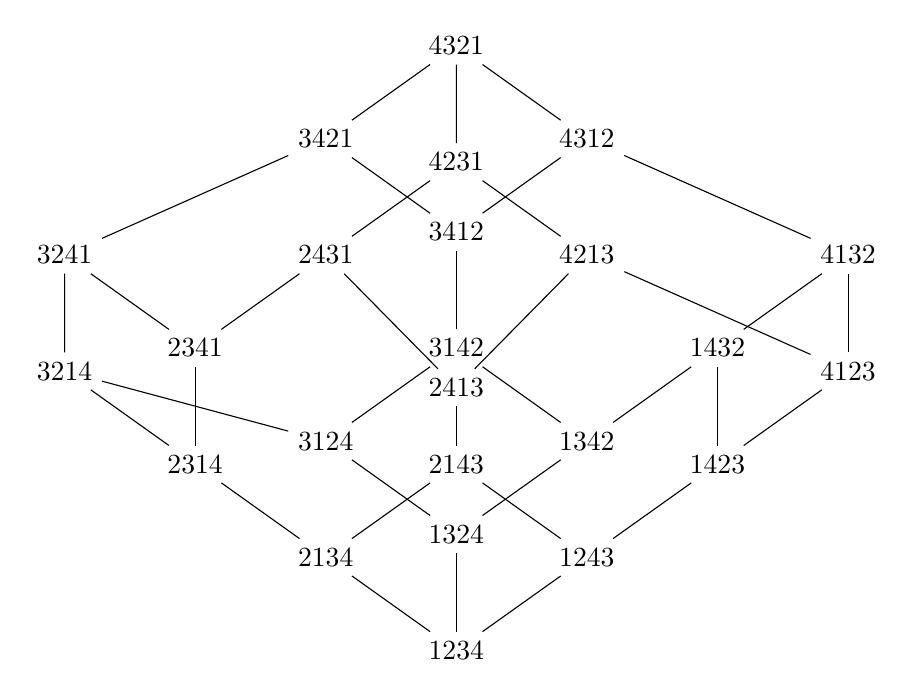
\begin{tikzpicture}
\node (1234) at (0,0) {1234};
\node[above left=1cm of 1234](2134) {2134};
\node[above=1cm of 1234](1324) {1324};
\node[above right=1cm of 1234](1243) {1243};
\node[above left=1cm of 2134](2314) {2314};
\node[above right=1cm of 2134](2143) {2143};
\node[above left=1cm of 1324](3124) {3124};
\node[above right=1cm of 1324](1342) {1342};
\node[above left=1cm of 2314](3214) {3214};
\node[above=1cm of 2314](2341) {2341};
\node[above=0.5cm of 2143](2413) {2413};
\node[above left=1cm of 1342](3142) {3142};
\node[above right=1cm of 1243](1423) {1423};
\node[above right=1cm of 1342](1432) {1432};
\node[above right=1cm of 1423](4123) {4123};
\node[above=1cm of 3214](3241) {3241};
\node[above right=1cm of 2341](2431) {2431};
\node[above=1cm of 3142](3412) {3412};
\node[above right=1cm of 3142](4213) {4213};
\node[above=1cm of 4123](4132) {4132};
\node[above left=1cm of 3412](3421) {3421};
\node[above right=1cm of 3412](4312) {4312};
\node[above left=1cm of 4213](4231) {4231};
\node[above=1cm of 4231](4321) {4321};
\draw (1234)--(2134);
\draw (1234)--(1324);
\draw (1234)--(1243);
\draw (2134)--(2314);
\draw (2134)--(2143);
\draw (1243)--(2143);
\draw (1324)--(3124);
\draw (1324)--(1342);
\draw (2314)--(3214);
\draw (2314)--(2341);
\draw (3124)--(3214);
\draw (3124)--(3142);
\draw (2143)--(2413);
\draw (1342)--(3142);
\draw (1342)--(1432);
\draw (1423)--(1432);
\draw (1423)--(1243);
\draw (4123)--(1423);
\draw (3214)--(3241)--(2341);
\draw (2341)--(2431)--(2413);
\draw (3142)--(3412);
\draw (3241)--(3421)--(4321)--(4312);
\draw (4321)--(4231)--(2431);
\draw (1432)--(4132)--(4312);
\draw (4123)--(4213)--(4231);
\draw (3421)--(3412)--(4312);
\draw (4123)--(4132);
\draw (4213)--(2413);
\end{tikzpicture}

\end{document}
